%!TEX root = main.tex
% \begin{figure}[htb]
% \begin{center}
% %optional pour enlever un peu d'espace blanc de votre silhouette
% %\vspace{-.3cm}
%  %\includegraphics[keepaspectratio,width=0.5\textwidth]{fig/nomde}
% % analoog
% %\vspace{-0.6cm}
%  % \caption{ici un logo}
%  % \label{fig:ruglogo}
% %analoog
% %\vspace{-.6cm}
% \end{center}
% \end{figure}

% Utilisation du template
% \cite(reference à citer)
% \ref(figure à référencer)

\chapter{Améliorations classiques des Réseaux de neurones appliqués à GAN}


\paragraph{}
Les réseaux de neurones que nous utilisons pour le GAN sont de simples perceptrons. De nombreuses méthodes pour améliorer les résultats et/ou la convergence ont été proposés pour ces types de réseaux. Nous avons étudié en particulier les algorithmes de descente de gradient avec pas adaptatif et les réseaux de neurones à convolution. 

\section{Algorithmes de descente de gradient à pas adaptatif}
\paragraph{}
En utilisant la descente de gradient classique, nous avons constaté que, dans le générateur, presque seule la couche de sortie travaillait. Le GAN ne générait alors pas des images d'assez bonne qualité ni assez diverses. Nous nous sommes donc intéressés à d'autres algorithmes de descente, dans l'espoir qu'ils soient plus efficaces et atteignent plus "en profondeur" les réseaux. 
\paragraph{}
Les algorithmes de descente auxquels nous nous sommes intéressés sont notamment des algorithmes à pas adaptatif. En effet, dans ces algorithmes, le pas change au fur et à mesure de l'apprentissage. Il peut être grand au début, pour aller dans la bonne direction, et petit à la fin pour plus de précision. 

\subsection{Momentum}
Dans une descente de gradient classique, la formule de mise à jour des poids est la suivante. 
\[W_{k+1} = W_k - \eta * \frac{\partial J}{\partial W}\]
On peut également le noter :
\[\Delta W_k = -\eta*\frac{\partial J}{\partial W}\]

Une première méthode qui est compatible avec tous les algorithmes suivants est de rajouter une inertie au gradient, ou momentum. Le but est de limiter les oscillations "inutiles" qui peuvent arriver lors d'une descente de gradient. On a alors : 
\[\Delta W_k  = \mu * W_k - \eta*\frac{\partial J}{\partial W}\]

\subsection{AdaGrad}
AdaGrad (qui signifie Adaptative Gradient) est un algorithme où le pas change en fonction de l'erreur. 
On calcule la somme des carrés des gradients : 
\[g_{k+1} = g_k + (\frac{\partial J}{\partial W})^2\]

La formule de mise à jour des poids est alors : 
\[\Delta W_k = -\frac{\partial J}{\partial W}*\frac{\eta}{\sqrt{g_{k+1}}+\epsilon}\]

$\epsilon$ est une valeur arbitrairement faible pour éviter une division par zéro et pour initialiser l'algorithme. L'inconvénient majeur de AdaGrad est que la quantité $g_k$ ne peut qu'augmenter dans le temps, ce qui implique que le pas devient de plus en plus faible. Si l'apprentissage dure trop longtemps, les poids ne bougeront presque plus à cause du faible pas.

\subsection{RMSProp}
RMSProp est sensiblement identique à Adagrad mais avec une amélioration : au lieu de considérer la somme des carrés des gradients, on considère une pondération de cette somme. Cela permet de donner plus d'importance aux derniers gradients. 
On calcule donc : 
\[g_{k+1} = \gamma*g_k + (1-\gamma)*(\frac{\partial J}{\partial W})^2\]

La formule de mise à jour des poids est donc identique à celle d'Adagrad : 
\[\Delta W_k = -\frac{\partial J}{\partial W}*\frac{\eta}{\sqrt{g_{k+1}}+\epsilon}\]

Dans le calcul de $g_k$, il y a un terme quadratique. On appelle donc $g_k$ \textbf{moment d'ordre 2}. Il existe également un moment d'ordre 1 qui se calcule par :
\[g_{k+1} = \gamma*g_k + (1-\gamma)*\frac{\partial J}{\partial W}\]
Cela donne comme équation de mise à jour des poids : 
\[\Delta W_k = -\frac{\partial J}{\partial W}*\frac{\eta}{\sqrt{g_{t+1}-(m_{t+1})^2}+\epsilon}\]


\subsection{Adadelta}
Cet algorithme est similaire à RMSProp et utilise également une somme mobile pour calculer le moment d'ordre 2 du gradient, $g_k$. Cependant, au lieu d'avoir un $\eta$ fixe, on introduit $x_k$, le moment d'ordre 2 de $\Delta W_k$.
\[g_{k+1} = \gamma*g_k + (1-\gamma)*(\frac{\partial J}{\partial W})^2\]
\[x_{k+1} = \gamma*x_k + (1-\gamma)*(\Delta W_k)^2\]

On obtient donc :
\[\Delta W_k = -\frac{\partial J}{\partial W}*\frac{\sqrt{x_k + \epsilon}}{\sqrt{g_{t+1}-(m_{t+1})^2}+\epsilon}\]
\subsection{Adam}
Adam (pour Adaptive Moment Estimation) adapte le pas en fonction des moments d'ordre 1 et 2 du gradient. Notons $m_k$ le moment d'ordre 1 et $v_k$ le moment d'ordre 2.
On les calcule par :
\[m_{k+1} = \beta_1*m_k + (1-\beta_1)*g_k\]
\[v_{k+1} = \beta_2*v_k + (1-\beta_2)*g_k^2\]

Quand $m_k$ et $v_k$ sont initialisés à 0, ils sont biaisés vers 0.
Pour pallier à cela, on considère $\widehat{m_k}$ et $\widehat{v_k}$ : 
\[\widehat{m_{k}} = \frac{m_k}{1-\beta_1^k}\]
\[\widehat{v_{k}} = \frac{v_k}{1-\beta_2^k}\]

On met à jour les poids avec :
\[\Delta W_k = -\frac{\eta}{\sqrt{\widehat{v_k}}+\epsilon}*\widehat{m_k}\]

\subsection{Comparaison des algorithmes sur MNIST}

	Sur la figure \ref{fig:comp_algos}, on voit que ces algorithmes améliorent le résultat sur MNIST autant en précision qu'en vitesse de convergence par rapport à l'algorithme de descente de gradient classique. Le meilleur algorithme à utiliser est Adam avec $\eta = 0.01$, $\gamma_1=0.9$ et $\gamma_2 = 0.999$ comme paramètres. Cependant, comme l'a étudié le groupe Couleuvre, il peut être avantageux d'utiliser deux algorithmes différents sur le générateur et le discriminateur. En effet, utiliser Adam sur le générateur et RMSProp sur le discriminateur permet de "ralentir" le discriminateur qui a tendance à devenir meilleur que le générateur. 
	
\begin{figure}[h!]
  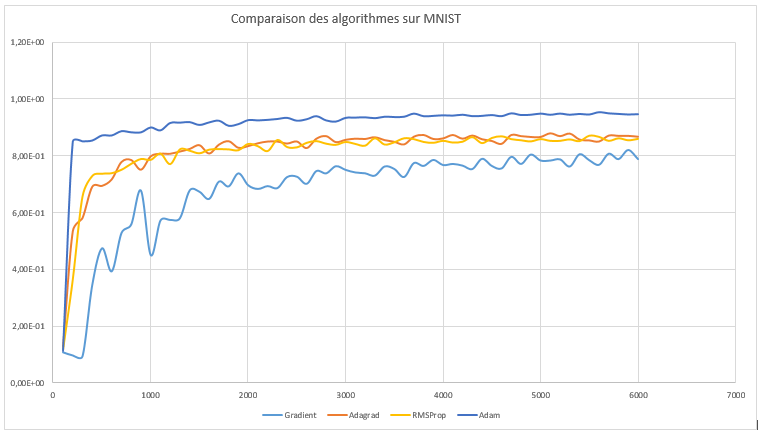
\includegraphics[width=\linewidth]{fig/comparaisonAlgos.png}
  \label{fig:comp_algos}
\end{figure}

\section{Réseaux à convolution: DCGAN}

Cette section sera remplie quand Romain finira par mettre sa partie du rapport en ligne.